% !TEX program = pdflatex
\documentclass[11pt,a4paper]{article}

% === PACKAGES (house style, mirrored from sbom-prune) ===
\usepackage[utf8]{inputenc}
\usepackage[T1]{fontenc}
\usepackage{lmodern}
\usepackage[margin=1in]{geometry}
\usepackage{setspace}
\usepackage{parskip}
\usepackage{graphicx}
\usepackage{float}
\usepackage{booktabs}
\usepackage{amsmath}
\usepackage{amssymb}
\usepackage{hyperref}
\usepackage{listings}
\usepackage{xcolor}
\usepackage{caption}
\usepackage{subcaption}
\usepackage{tikz}
\usepackage{pgfplots}
\pgfplotsset{compat=1.18}

% === CODE LISTING STYLE ===
\definecolor{codegreen}{rgb}{0,0.6,0}
\definecolor{codegray}{rgb}{0.5,0.5,0.5}
\definecolor{codepurple}{rgb}{0.58,0,0.82}
\definecolor{backcolour}{rgb}{0.95,0.95,0.92}

\lstdefinestyle{mystyle}{
    backgroundcolor=\color{backcolour},
    commentstyle=\color{codegreen},
    keywordstyle=\color{magenta},
    numberstyle=\tiny\color{codegray},
    stringstyle=\color{codepurple},
    basicstyle=\ttfamily\footnotesize,
    breakatwhitespace=false,
    breaklines=true,
    captionpos=b,
    keepspaces=true,
    numbers=left,
    numbersep=5pt,
    showspaces=false,
    showstringspaces=false,
    showtabs=false,
    tabsize=2
}
\lstset{style=mystyle}

% === TITLE INFO ===
\title{
    \vspace{-2em}
    \rule{\textwidth}{1pt}\\[0.5em]
    \textbf{Static-GTFS Bus ETA for Delhi}\\[0.3em]
    \large What a Timetable Alone Can and Cannot Tell Riders\\[0.5em]
    \rule{\textwidth}{1pt}
}
\author{
    Ashay Kushwaha\\
    \textit{CypherLabs Open Research}\\
    \texttt{https://github.com/AshayK003/gtfs-eta}
}
\date{September 2026}

\begin{document}

\maketitle

\begin{abstract}
Most Indian city buses have no live display, and real-time vehicle-location feeds barely exist. The default deployment is a static timetable---and the static feed itself models no delay: intervening stop times are constant-speed estimates with arrival equal to departure everywhere. We ask what rider value a static timetable alone can still deliver, on a frozen Delhi cluster (routes 159UP/159DOWN, 316 trips, 9006 stop-times). First, a negative result with proof: per-segment travel times have \textbf{zero variance} feed-wide (3.27M rows, 115,752 segments, none above 1\,s std), so any static-only learning collapses to timetable lookup---a planned Kalman/GBM ladder was deleted before printing its first zero. Second, the positive result: scheduled \textit{headways} do vary, and classical waiting-time math turns them into honest expected waits (3.4--4.8\,min across dayparts, CV $\approx$ 0.5--0.6), packaged with next-departure lookup in a fully offline tool. Every number regenerates with one command from a committed 345\,KB cluster slice.
\end{abstract}

\vspace{1em}
\noindent\textbf{Keywords:} GTFS static, bus arrival time, headways, waiting time, Delhi, offline ETA

\newpage
\tableofcontents
\newpage

\section{Introduction}

A rider at a Delhi bus stop wants one number: how long until my bus. Where live displays and vehicle-location feeds exist, the answer comes from real-time systems. Across most Indian cities they do not exist, and the fallback is a printed timetable or nothing. The research literature largely aims elsewhere---graph neural networks and LSTMs that assume the dense automatic-vehicle-location data missing here, or commercial dashboards that assume fleet hardware.

This report takes the deployment constraint literally: \textit{static timetable in, rider answers out, no connectivity, no learning from observations that do not exist.} On a frozen Delhi cluster we measure exactly what the timetable contains. The headline is a split verdict. What it does \textit{not} contain is any variance to learn from---a finding we prove feed-wide rather than assume. What it \textit{does} contain is headway structure, which converts via textbook waiting-time math into expected waits that beat naive half-headway rules by accounting for scheduled irregularity. Contributions:

\begin{itemize}
    \item A frozen, fully offline-reproducible Delhi cluster (345\,KB committed slice of a 19.8\,MB mirrored feed) with integrity validation.
    \item A feed-wide zero-variance proof that deletes an entire modeling ladder before it wastes work---reported as a finding, not a failure.
    \item Per-daypart headway and expected-wait tables plus a working offline lookup package (next departures + expected wait).
    \item An honest static ceiling with a built-in evaluation seam for real-time scoring when keyed data arrives.
\end{itemize}

\section{Background and Related Work}

\subsection{Schedule-based transit data and its limits}

Schedule-based GTFS accessibility work has repeatedly found that timetables overstate reality: Wessel \& Farber (2019) estimate 5--15\% overstatement of accessibility from schedules alone, and Newmark (2024) documents how agencies code constant times for intervening stops with arrival equal to departure everywhere---no dwell modeling, no variance. Our feed matches that description exactly (Section~\ref{sec:results}), which makes this report a worked example of building honestly inside those limits rather than around them.

\subsection{Delhi feeds}

Delhi's Open Transit Data portal (Govt.\ of NCT Delhi with IIIT-Delhi) publishes static timetables (3464 stops, 543 routes, June 2024) and key-gated real-time data. In practice, the origin host was unreachable at measurement time and a commercial mirror was key-gated; the frozen snapshot used here comes from the Mobility Database mirror (mdb-3139/mdb-1262, byte-identical, 19.8\,MB), which itself archives the Delhi feed. Bengaluru's BMTC mirror (daily-fresh, 4434 routes) was surveyed as a transfer candidate but at 195\,MB unzipped exceeds the size budget---transfer checks stay sampled. Existing Delhi analyses are descriptive (coverage statistics, EDA plots); none ship prediction.

\subsection{ waiting-time math}

For random passenger arrivals, expected wait relates to headways by $E[w] = E[h]/2 + \mathrm{Var}(h)/(2E[h])$: perfectly regular service halves the mean headway, while irregularity adds a variance penalty. The formula needs only scheduled departures, making it the correct tool for static-only analysis---unlike delay prediction, which needs observations.

\section{Methodology}

\subsection{Parser and integrity}

\verb!gtfs_parse.py! (pandas) reads the five core GTFS files with all columns as strings (ids keep leading zeros; times past 24h parse to seconds) and reports referential integrity: orphan stop/trip/route ids and tripless trips. The frozen feed validates fully clean (Section~\ref{sec:results}).

\subsection{Zero-variance proof method}

Per-segment travel time (next arrival minus current arrival) is aggregated per (route, from-stop, to-stop) across trips with a streaming pass (Welford accumulators, 3.27M rows); any segment with standard deviation above 1\,s would refute the claim. Arrival equals departure is checked separately on a 200k-row sample. Both the cluster and the full feed are measured.

\subsection{Headways and lookup}

Trip starts (first departures) per route are sorted into gaps; per (route, daypart) buckets we report trip count, mean $\pm$ std headway, coefficient of variation, and expected wait. Gaps over 2\,h count as service breaks (e.g.\ the overnight halt): excluded from wait math, counted in the table---a 313-minute ``expected wait'' at 3am was caught and fixed during development, and the rule exists so it cannot recur. \verb!lookup.py! answers next-$k$ departures plus expected wait from timetable and headway table only.

\subsection{Corpus and freeze policy}

\verb!corpus.json! v1 freezes the feed fingerprint, full inventory, and the cluster choice (DTC 159UP/159DOWN, routes 5064/5530, 316 trips: the densest balanced directional pair, single agency). The 345\,KB cluster slice ships in \verb!data/cluster/!; the full 19.8\,MB zip stays local and ignored.

\subsection{Blind spots}

Constant-speed stop times (nothing observed to learn); arrival = departure (no dwell signal); single-cluster scope; schedule-shaped analysis until keyed real-time data lands (stated, not hidden); headway math assumes random arrivals during service hours.

\section{Results}
\label{sec:results}

One command (\verb!python evaluate.py!) regenerates everything below from the committed slice, no downloads.

\subsection{Integrity and the zero-variance proof}

Integrity: 0 orphan stops, 0 orphan trips, 0 tripless trips, 0 orphan routes. Variance: 55 cluster segments with max std \textbf{0.0\,s}; feed-wide, 115,752 segments with \textbf{none above 1\,s}. Dwell check: 0 of 200,000 sampled rows differ. The static feed is perfectly self-consistent constant-speed estimates at second resolution (e.g.\ 06:01:13, 06:07:27)---granular, but identical on every trip.

\subsection{Headways and expected waits}

\begin{table}[H]
\centering
\caption{Headway statistics and expected wait per route and daypart (minutes).}
\label{tab:headways}
\begin{tabular}{@{}llrrrr@{}}
\toprule
Route & Bucket & Trips & Headway & CV & E[wait] \\
\midrule
5064 (159UP) & morning-peak & 43 & 5.43$\pm$2.78 & 0.512 & 3.43 \\
5064 (159UP) & midday & 44 & 6.93$\pm$4.37 & 0.630 & 4.84 \\
5064 (159UP) & evening-peak & 38 & 6.27$\pm$3.82 & 0.609 & 4.30 \\
5064 (159UP) & off & 33 & 6.48$\pm$3.33 & 0.514 & 4.10* \\
5530 (159DOWN) & morning-peak & 42 & 5.61$\pm$2.75 & 0.490 & 3.48 \\
5530 (159DOWN) & midday & 44 & 6.77$\pm$4.08 & 0.603 & 4.61 \\
5530 (159DOWN) & evening-peak & 41 & 5.80$\pm$3.22 & 0.555 & 3.79 \\
5530 (159DOWN) & off & 31 & 6.83$\pm$3.81 & 0.557 & 4.47* \\
\bottomrule
\end{tabular}
\end{table}

(* off-bucket waits exclude one overnight service break each, counted not averaged.)

\begin{figure}[H]
\centering
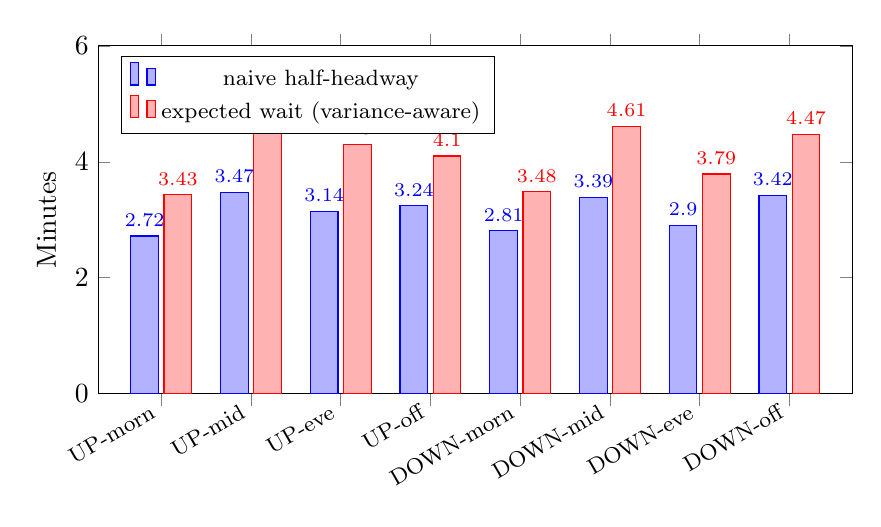
\begin{tikzpicture}
\begin{axis}[
    ybar, width=0.92\textwidth, height=6cm,
    symbolic x coords={UP-morn,UP-mid,UP-eve,UP-off,DOWN-morn,DOWN-mid,DOWN-eve,DOWN-off},
    xtick=data, x tick label style={rotate=30, anchor=east, font=\footnotesize},
    ymin=0, ymax=6, ylabel={Minutes},
    legend pos=north west, legend style={font=\footnotesize},
    nodes near coords, nodes near coords style={font=\scriptsize},
]
\addplot coordinates {(UP-morn,2.72) (UP-mid,3.47) (UP-eve,3.14) (UP-off,3.24) (DOWN-morn,2.81) (DOWN-mid,3.39) (DOWN-eve,2.90) (DOWN-off,3.42)};
\addlegendentry{naive half-headway};
\addplot coordinates {(UP-morn,3.43) (UP-mid,4.84) (UP-eve,4.30) (UP-off,4.10) (DOWN-morn,3.48) (DOWN-mid,4.61) (DOWN-eve,3.79) (DOWN-off,4.47)};
\addlegendentry{expected wait (variance-aware)};
\end{axis}
\end{tikzpicture}
\caption{Naive half-headway versus variance-aware expected wait: scheduled irregularity (CV $\approx$ 0.5--0.6) costs riders roughly an extra minute over the naive rule, consistently across routes and dayparts.}
\label{fig:waits}
\end{figure}

\begin{figure}[H]
\centering
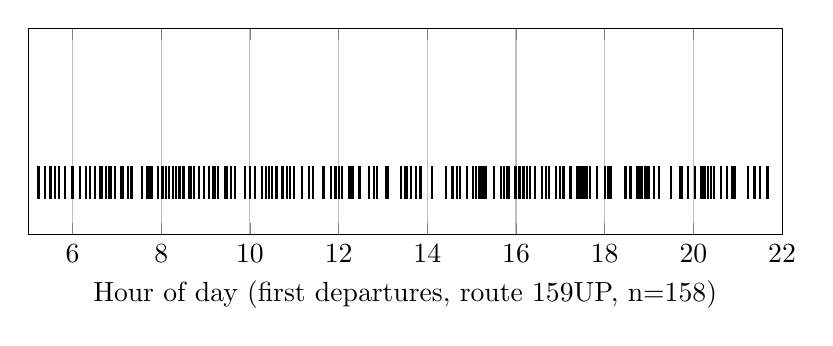
\begin{tikzpicture}
\begin{axis}[
    width=0.92\textwidth, height=4.2cm,
    xmin=5, xmax=22, ymin=-0.5, ymax=1.5, ytick=\empty,
    xlabel={Hour of day (first departures, route 159UP, n=158)},
    grid=major,
]
\addplot[only marks, mark=|, mark size=6pt, thick] coordinates {
(5.23,0) (5.37,0) (5.50,0) (5.60,0) (5.70,0) (5.83,0) (6.00,0) (6.17,0) (6.30,0) (6.40,0) (6.50,0) (6.63,0) (6.67,0) (6.75,0) (6.83,0) (6.87,0) (6.95,0) (7.10,0) (7.13,0) (7.25,0) (7.33,0) (7.57,0) (7.67,0) (7.70,0) (7.73,0) (7.78,0) (7.93,0) (8.03,0) (8.10,0) (8.17,0) (8.27,0) (8.33,0) (8.40,0) (8.42,0) (8.50,0) (8.62,0) (8.67,0) (8.73,0) (8.85,0) (8.97,0) (9.08,0) (9.17,0) (9.20,0) (9.28,0) (9.43,0) (9.47,0) (9.58,0) (9.67,0) (9.88,0) (10.00,0) (10.12,0) (10.27,0) (10.37,0) (10.43,0) (10.50,0) (10.60,0) (10.73,0) (10.75,0) (10.83,0) (10.90,0) (11.00,0) (11.17,0) (11.33,0) (11.42,0) (11.65,0) (11.67,0) (11.83,0) (11.93,0) (12.00,0) (12.08,0) (12.23,0) (12.27,0) (12.33,0) (12.47,0) (12.68,0) (12.80,0) (12.87,0) (13.08,0) (13.10,0) (13.40,0) (13.50,0) (13.55,0) (13.63,0) (13.75,0) (13.83,0) (13.85,0) (14.10,0) (14.42,0) (14.57,0) (14.67,0) (14.73,0) (14.90,0) (15.03,0) (15.10,0) (15.17,0) (15.22,0) (15.27,0) (15.33,0) (15.50,0) (15.67,0) (15.73,0) (15.80,0) (15.83,0) (15.97,0) (16.00,0) (16.08,0) (16.17,0) (16.18,0) (16.25,0) (16.32,0) (16.43,0) (16.58,0) (16.67,0) (16.75,0) (16.90,0) (17.00,0) (17.07,0) (17.23,0) (17.37,0) (17.43,0) (17.50,0) (17.55,0) (17.60,0) (17.67,0) (17.83,0) (18.00,0) (18.07,0) (18.13,0) (18.47,0) (18.58,0) (18.72,0) (18.77,0) (18.83,0) (18.92,0) (18.98,0) (19.00,0) (19.12,0) (19.23,0) (19.50,0) (19.70,0) (19.75,0) (19.87,0) (20.03,0) (20.17,0) (20.23,0) (20.25,0) (20.33,0) (20.40,0) (20.47,0) (20.63,0) (20.75,0) (20.87,0) (20.92,0) (20.93,0) (21.23,0) (21.38,0) (21.50,0) (21.67,0)};
\end{axis}
\end{tikzpicture}
\caption{First departures across the service day (route 159UP, 05:14--21:40): dense daytime service with visibly irregular spacing, then the overnight halt. Irregularity is the entire content of Table~\ref{tab:headways}.}
\label{fig:rug}
\end{figure}

Peaks run $\sim$5.5-minute headways, midday $\sim$6.8; CV sits 0.49--0.63 in every bucket, so expected waits exceed naive half-headways by roughly a minute throughout. Off-peak headways match daytime levels---DTC runs route 159 frequently across all service hours, with exactly one overnight break per direction.

\subsection{Lookup demo}

Route 5064, stop 3075, after 08:00 $\to$ next 08:02, 08:06, 08:10 with E[wait] 3.43\,min; mid-route stop 535 after 18:00 $\to$ 18:00, 18:04, 18:07 with E[wait] 4.30\,min. Timetable plus headway table only; no connectivity, no weights.

\section{Discussion}
\label{sec:discussion}

\subsection{Key findings}

First, the negative result is load-bearing: zero variance across 115,752 segments means delay \textit{prediction} from static data is vacuous, and any paper-shaped claim otherwise would be fitting noise. Reporting it---with the deleted ladder as evidence of process---is more useful than a table of zeros. Second, the positive result is genuinely rider-facing: irregular scheduled headways cost $\sim$1\,min over naive expectations, and the lookup package turns that into per-stop answers. Third, feed forensics (dead origin host, gated commercial mirror, byte-identical community mirrors) belongs in the methods section of civic-tech work, not in a footnote: reproducibility starts at acquisition.

\subsection{Limitations}

Single cluster (316 trips); headway math assumes random arrivals during service; scheduled---not observed---times throughout, so all waits are timetable-structure statements until keyed realtime data arrives; BMTC transfer unmeasured (sample local only); map-matching deferred, so stop coordinates are taken as given.

\subsection{Future work}

In priority order, as filed in the repository's contributing guide: (1) city-wide modeling beyond the frozen cluster; (2) realtime scoring through the built evaluation seam; (3) BMTC sampled transfer; (4) map-matching if coordinates prove unreliable.

\section{Conclusion}

On a frozen Delhi cluster, a 300-line standard-library package with a strict measure-first loop proves the static feed contains no learnable variance, then extracts what it does contain: headway structure worth $\sim$1\,min of honest expected wait over naive rules, packaged as an offline lookup tool. The work's secondary contribution is procedural: let feed-wide measurement---not modeling ambition---decide what gets built, and report the deleted ladder alongside the shipped one.

\section{Reproducibility}
\label{sec:repro}

\subsection{Installation}

No dependencies beyond CPython $\ge$ 3.10, pandas, numpy, and pytest for the suite. The 345\,KB cluster slice ships in the repo; the full 19.8\,MB feed stays local.

\subsection{Run benchmarks}

\begin{lstlisting}[language=bash]
git clone https://github.com/AshayK003/gtfs-eta.git
cd gtfs-eta
python -m pytest tests -q   # 6 passed: parser, headways, lookup
python evaluate.py          # committed slice: proof, headways, demo
python evaluate.py data/delhi.zip  # full-feed re-run (MobilityDB mdb-3139)
\end{lstlisting}

The suite checks parsing against a hand-computed micro-feed, headway math against closed forms, and lookup against known answers---hermetic, no network.

\subsection{Repository structure}

\verb!corpus.json! (frozen feed fingerprint, inventory, cluster choice), \verb!gtfs_parse.py! (tidy tables + integrity), \verb!headways.py! (stats + expected wait), \verb!lookup.py! (offline package), \verb!evaluate.py! (one-command report), \verb!tests/! (the runnable checks), \verb!data/cluster/! (committed slice), \verb!internals/! (working notes, not published except this report).

\begin{thebibliography}{9}

\bibitem{wessel} Wessel, N. \& Farber, S. On the accuracy of schedule-based GTFS for measuring accessibility. \textit{JTLU} 2019. \url{https://doi.org/10.5198/jtlu.2019.1502}

\bibitem{newmark} Newmark, G. Assessing GTFS Accuracy. Mineta Transportation Institute, 2024. \url{https://doi.org/10.31979/mti.2024.2017}

\bibitem{otd} Open Transit Data, Delhi (Govt.\ of NCT Delhi + IIIT-Delhi). \url{https://otd.delhi.gov.in/data/static/}

\bibitem{mobdb} Mobility Database (mirror mdb-3139/mdb-1262, validator reports). \url{https://mobilitydatabase.org/}

\bibitem{bmtc} Vonter/bmtc-gtfs (BMTC unofficial mirror, transfer candidate). \url{https://github.com/Vonter/bmtc-gtfs}

\bibitem{busmaps} busmaps.com dimts build (validation reference). \url{https://busmaps.com/en/india/Open-Transit-Data-DELHI/dimts}

\end{thebibliography}

\end{document}
